%\documentclass[iop,revtex4,apj]{emulateapj}
\documentclass[iop,revtex4]{emulateapj_mod}
%\usepackage{natbib}
\usepackage{amsfonts}
\usepackage{amssymb}
\usepackage[printonlyused]{acronym}
%\usepackage{amsmath,amsthm}
\usepackage{enumerate}
\usepackage{amsmath, amssymb, mathrsfs}
\usepackage{rotate}
\usepackage{lscape}
%\bibliographystyle{plain} 
\begin{document}
%Title Page: The first page of your report should be the signed Pre-lab Discussion page that was the first page of your lab manual.
\title{Brownian Motion in Cells}
\author{Jung Lin (Doris) Lee [Partner: Xiyue Wang] }
 \begin{abstract}
  We investigated solutions of different microbead size and viscosity in order to test whether the Einstein-Smoluchowsky equation holds true. We track particles undergoing Brownian diffusion using a microscope and record their position, displacement, and velocity information. Using this information, we compute the diffusion coefficients of different solutions and found that they agree with the  theoretical estimates of the diffusion coefficient, which depended on the particle size and viscosity. The linear fit analysis method yielded experimental diffusion coefficients that were on average 24.89$\pm 0.157$\% close to the theoretical estimates. However, using both the direct method and the Gaussian-fitting method, our analysis of the diffusion coefficient from the experimental values yielded an order of magnitude discrepancy from the theoretical values. We also analyzed the motion for a  molecular protein in a onion cell sample undergoing active intracellular transport, which had a non-Gaussian velocity distribution averaged around  at around v = 2.569$ \pm 1.011 \mu m/s$.
%  7.04,57.7,1.0284,26.987,31.679
 \end{abstract}
\nocite{*} 
\section{Introduction}\label{sec:intro}
 %Introduction: This should describe the physics and give an overview of what you are going to do. Aim to answer the questions: Why would someone want to do this experiment? What is gained?
 %motion from matter composed of atmons  to collide with each other
\par Brownian motion describes the random motion of small, free particles in a fluid medium due to their kinetic motion.  Albert Einstein's theoretical formulation of Brownian motion and Jean Perrin's experimental work were significant because it served as the one of the first experimental evidence for the  atomic nature of matter. The statistical theory of  random walk is crucial for the study of Markov process (i.e. random processes that do not depend on their past history),which is often used for modelling real-world systems such as the financial market and population genetics. %\citep{wiki_markov}  
\par In this experiment, we used a Zeiss Axiovert 200 microscope to look at particles undergoing Brownian motion. We track the particle's motion in order to compute an experimental value for the diffusion coefficient. We vary the viscosity, bead size, and solution type to examine whether the different resulting diffusion coefficient agrees with the relation derived from Langevin's equation and our intuition from the kinetic molecular theory(KMT). Finally, we observe an onion cell under the microscope to observe intracellular transport and the motion of molecular motors.
% We use the ----- compare with the random walk Brownian motion.
%theory, procedure, analysis 
\par In this report, we present the experimental methods and analysis used to obtain the diffusion coefficients for various particle size and viscosity. In section 2, I will present the theory behind Brownian diffusion by introducing the Einstein-Smoluchowsky equation and our experimental hypothesis. In section 3, I will detail the experimental setup and procedure of the experiment. Finally, in section 4,  I will present our analysis of the experimental data and how we obtained diffusion coefficients using two different methods and the average velocity of the molecular motor . We find that even though the experimental value of the diffusion coefficient obtained from the linear fit agreed very well with simulation, the diffusion coefficient computed using the direct method and Gaussian method in our analysis did not agree with the expected value due to the noise in the collected data.

\section{Theory}\label{sec:theory}
%Theory: Include the working equations that you will be using but do not include lengthy derivations (such as the Compton or Rutherford formulas) unless specifically asked.where the equations come from and what they are dependent on, (assumptions, conservation laws, etc.), cite reference 
\subsection{Basics}
\par In Einstein's original 1905 derivation, he combined the equations that describes osmotic pressure with a series of equations that describes how particles moves through viscous fluids to calculate the theoretical value of the diffusion coefficient, a dimensionless number that describes the extent to which a particle is freely diffusing through the medium without any obstruction \citep{einstein_1905}\footnote{A more simplified derivation can be found in  \cite{newburgh},\cite{einstein_langevin}.}. Since Brownian motion is a series of random walks, it can be modeled as a normal distribution, which means that we can look at the denominator of its exponent to get the variance of the distribution\citep{math}. This mean squared displacement for a list of particle positions, either obtained through simulation or experiment, can also enable us to compute the value of D. As derived in Einstein's 1905 paper, the Einstein-Smoluchowsky equation is as follows
\begin{equation}
D = \sqrt{\langle |\vec{r}(t+\tau)-\vec{r}(t) |\rangle ^2 /2d\tau}
\label{exp}
\end{equation}
where d is the number of dimensions, $\tau$ is the sampling time (0.1 s).
\par For a free particle, diffusing in a Newtonian fluid, the diffusion coefficient is defined as : 
\begin{equation}
D \equiv \frac{k_bT}{3\eta r}
\label{theory}
\end{equation}
where $k_b$ is the Boltzman's constant, T is temperature, $\eta$ is the viscosity of the solution and r is the radius of the particle. Despite the complex derivations, this formula  makes intuitive sense in terms of the familiar kinetic molecular theory(KMT): as the temperature is higher or if the particle size is small, the velocity of the particles are higher, thus the particles collides more rigorously and frequently and more diffusion occurs;  as the solutions gets more viscous, the solution effectively slows the particles down so less diffusion occurs.

\subsection{Simulation}\label{sim}
For the particle simulation,  (using code provided in the worksheet) we first create a vector of random steps. We then compute the theoretical D using Eq.\ref{theory} to obtain an amplitude (k=$\sqrt{2dD\tau}$, where d = dimensions) for scaling up the random steps. Then using these simulated particle positions, we estimate the value of D using Eq.\ref{exp}. Because this is a stochastic process, the error depends on $1/\sqrt{N}$, a more detailed error propagation yields the uncertainty quoted in the simulated D values. We used a temperature of 20 degrees Celsius, comparable to our experimental conditions. There is some uncertainty in the temperature because we record only the ambient room temperature and neglect any external heating of the sample due to the microscope light source. However, effects of heating from the microscope should be minimized by our Kohler Illumination setup.
\subsection{Hypothesis}\label{hypo}
 We chose to conduct our experiment on  5 different samples, summarized in Table  \ref{table} . Sample \#2 and \#3 enable us to test the effect of viscosity on the Brownian motion, while keeping the particle type and size the same. According to Eq.\ref{sec:theory} and our intuition from KMT, as the viscosity gets larger, there is less random motion and thus Sample \#3 should have a lower value of D.  Sample \#2 and \#4 enable us to compare the particle sizes, and we could similarly infer that Sample \#4 will have a lower value of D. Sample \#2 and \#4 enable us to compare the particle type. While the particle type is not explicitly a variable inside Eq.\ref{sec:theory}, we believe that since glycerol particles are more massive than PVP particle, it will result in slower random walk and therefore a lower value of D. The reasoning behind these experimental choices is that we are only changing one variable per comparison so that we know that the Sample \#2  serve as a standard for comparison. We also chose particle sizes small enough in the range suggested by the lab worksheet so that Brownian motion can actually be observed.
\section{Apparatus and Procedure}\label{sec:ap}
In this experiment we use an inverted compound microscope that is connected to a CCD camera where the image processing is done by a given particle tracking script. Following the procedures:
\begin{enumerate}
\item Set up Kohler Illumination ,dark field illumination and calibrate the microscope, as described in Sec. \ref{kohler}.
\item Prepare polyesterine microbead solution by first creating a stock solution and then diluting it to the appropriate amount (as solute and solvent proportions indicated in Table \ref{solution}), then put these on the microscope slides.
\item Observe the microbeads undergoing Brownian motion using the particle tracking software (Sec \ref{track}).
\item Prepare a slide of onion cell membrane (preferably near the core of the onion where there is more activity), and observe intracellular transport.
\end{enumerate}
\begin{figure}[h]
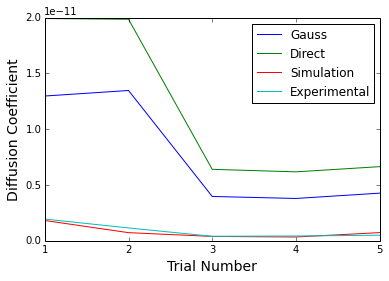
\includegraphics[width=0.40\textwidth]{plots/analysis.png}
\caption{The diffusion coefficient obtained from the Gaussian and direct method follows simmilar trends. This is about an order-of-magnitude off from the simulation and experimental results.}
\label{analysis4}
\end{figure}

\begin{figure}[h]
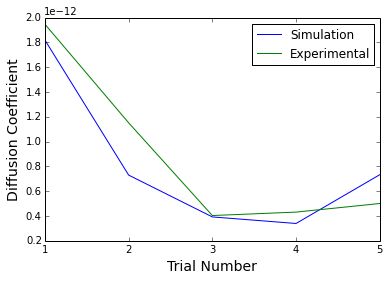
\includegraphics[width=0.40\textwidth]{plots/exp_sim.png}
\caption{The diffusion coefficient obtained from the simulation and the experiment follows the same trends for different trials, which makes sense in terms of the variables being changed as described in Sec.\ref{hypo} . }
\label{analysis4}
\end{figure}

\begin{table*}[t]
\centering
\caption{Experimental condition and results of all trials. ``Simulation" indicates the diffusion coefficient computed from a Matlab simulation of N=1000 particles undergoing random walk, as described in Sec. \ref{sim}.``Experimental" indicates the diffusion coefficient computed from the particle tracking interface. }
\label{my-label}
\begin{tabular}{llllll} \label{table}
Trial & Solution Type & Solution viscocity\footnote{The uncertainty on the solution viscosity and microbead size are not given in the datasheet.} [cp] & Microbead diameter [$\mu m$] & Simulation D          & Experimental D \\
1     & $H_2O$         &  1.00                           & 0.47                              & $1.8184\times 10^{-12}\pm 7.7701\times 10^{-15}$ & $1.9464\times 10^{-12}$     \\
2     & PVP           & 2.50                        & 0.47                              & $7.2988\times 10^{-13}\pm3.2730\times 10^{-15}$ & $1.1515\times 10^{-12}$     \\
3     & PVP           & 4.65                        & 0.47                              & $3.9260\times 10^{-13}\pm1.6801\times 10^{-15}$ & $4.0377\times 10^{-13}$     \\
4     & PVP           & 2.50                        & 1.01                              & $3.3975\times 10^{-13}\pm1.4979\times 10^{-15}$ & $4.3144\times 10^{-13}$     \\
5     & glycerol      & 2.50                        & 0.47                              & $7.3291\times 10^{-13}\pm3.2063\times 10^{-15}$ & $5.0073\times 10^{-13}$    
\end{tabular}
\end{table*}
\begin{table}[]
\centering
\caption{Recipe for making viscous solutions}
\label{solution}
\begin{tabular}{lllll}
viscosity[cp] & Type & solute:water & water[ml] & solute[g] \\
 2.50      & PVP         & 1:99         & 5.050 & 0.051  \\
 4.65      & PVP         & 2:98         & 4.020 & 0.082  \\
 2.50      & glycerol    & 32.2:67.8    & 1.611 & 0.765 
\end{tabular}
\end{table}

\subsection{Particle Tracking Code} \label{track}
\par Particle tracking code receives a stream of imaging data from the camera. Then, the BlobFinder uses a friends-of-friends algorithm for finding centroids by examining the intensities of neighboring pixels around outlier pixels  where the particle  are centered. We find that there is a short ($\approx$ 5 s) delay time between when a change on the microscope slide can be displayed on the computer screen due to the program's non-uniform sampling rate.
\par We modify the minimum particle size to correspond with the size of the microbead that we were observing.  If we were allowed to adjust the C\# source code, we would adjust the acceptable range of values for the minimum particle size so that we can increment smaller steps and more finely filter out the non-microbead motions; currently, the existing implementation only allow integer values to be entered in this text field. 
The data output contains the positional information (x,y) and the changes in time and position (dx, dy, dt) of each detected particles. In addition,  the displacement-squared $dr^2$, and a running total of the displacement squared $\Sigma dr^2$ where $dr = \sqrt{dx^2+dy^2}$ is also recorded. The pixel-to-meters conversion has already been applied to the data output and so the quantities in the resulting data file is in SI units.
\subsection{Microscope setup}\label{kohler}
\par  We adjust our condenser irises and depth of field to achieve Kohler Illumination to control the amount of light and the incident angle that the light shines on the sample. \footnote{Although not mentioned in the lab manual, we find it important in the initial setup to also adjust the intensity of the light source using the voltage button near the eyepiece.} This setup ensures that the image of the light source is not superposed onto the actual image of the specimen and provides uniform illumination and heating to the sample.  
\par Then we adjust the condenser so that so that all the illuminating light is blocked off and we only see the light that scatters off the specimen. This technique is called darkfield illumination and it enables us to look at small particles ($\leq1\mu m$ with the 40x objective) that would otherwise be hard to see with direct illumination.
\par To calibrate the microscope, we make a solution of 10.11$\mu \pm 0.703$ m Polystyrene microbeads and water to obtain a pixel-to-meters ratio used in the image-processing script. Since the pixel counting is an error-prone task, we counted the pixel of 3 particles and had both lab members count it, which yields a total of six values, then we averaged these to get an pixel to ratio conversion of 0.48 $\pm 0.15\mu m/$pixel for the 20x objective and 0.28$\pm 0.1 \mu m/$pixel for the 40x objective. (This makes intuitive sense because twice the magnification approximately yields half the pixel ratio.) The error is estimated on assuming uncertainty in pixel count of two pixels and propagated through the averaging of our six data points.
%Apparatus and Procedure: You should have enough detail so that one familiar with physics but not with the particular experiment at hand could reproduce your experiment if necessary. A block diagram of the equipment is essential here—this should be your own, and not copied out of a book or lab manual. Explain the major pieces of equipment and what they do, but do not overwhelm your reader with details here!
\section{Analysis}\label{sec:analysis}
%Analysis:  the calculations that the lab manual asks you to do are supposed to act as a guide to your analysis, and not as a series of separate calculations. agree with prediction? error analysis? source of error, uncertainty?  
\par For my analysis, I loaded in the experimental data using the given script \texttt{BrownianMotionParse} and used the Matlab function \texttt{BrownianMotionParse} to write out the parsed data into a textfile. All subsequent dataprocessing is conducted with Python. 
\subsection{Computing diffusion coefficient}\label{compD}
\par A Newtonian fluid is a fluid that has a simple fluid flow behavior where the shear stress is linearly proportional to the viscosity and the shear rate, which means that its viscosity only depends on temperature. The derivation of the diffusion coefficient assumes that the particle is freely diffusing in a Newtonian fluid  \cite{Philipse}, so this is why the solutions (water, gyleral and PVP)  we used in this experiment are all Newtonian. This gives us the relationship between viscosity, particle size, and diffusion coefficient as described in Sec. \ref{sec:theory}. 
\par From the Newtonian fluid assumption, we can use Newton's second law and model the force term as a frictional force that depends linearly on the viscosity. This gives us the Langevin equation (Eq. \ref{lang}), where the first term comes from the Newtonian derivation (ignoring the term for the random density perturbation in the fluid).
\begin{equation}
\frac{d^2x}{dt^2} = \frac{\gamma}{m}\frac{dx}{dt}
\label{lang}
\end{equation}where $\gamma  = 6\pi \eta a$.
Solving this differential equation yields the solution of form :
\begin{equation}
v(t) = e^{-t/\tau_B} v(0)
\end{equation}
\par We ignore the exponential component of the general solution because if we do a detailed calculation, we will find that Brownian motion is essentially a Markov (i.e. random) process, because there are as much as $10^{11}$ collisions during the 0.1 seconds time period that we are sampling that the effects of any interparticle correlation or interaction due to an external potential will not sustain. 
I computed the autocorrelation by computing the correlation between two adjacent positions:
\begin{equation}
corr(k) = \Sigma^N_{i=1} x_{i} * x_{i+k}
\end{equation} and obtained an average correlation of -0.00792$\pm $0.12525 to confirm that the diffusion process is largely random. The small nonzero autocorrelation may result from bulk flow due to uneven heating or elevation of the microscope slides. 
\begin{table}[]
\centering
\caption{Table of analysis values.``Direct", ``Linear",  and ``Gauss" indicates that the diffusion coeffcient computed by the method described in Sec. \ref{compD}. }
\label{table_analysis}
\begin{tabular}{lllll}
Trial & Direct     & Linear& Gauss      \\
1     & $1.9918\times10^{-11}$ & $2.3135\times 10^{-12}$ & $1.2973\times 10^{-11}$ \\
2     & $1.9852\times10^{-11}$ & $8.3564\times 10^{-13}$ & $1.3468\times10^{-11}$ \\
3     & $6.4042\times10^{-12}$ & $4.1256\times 10^{-13}$ & $3.9731\times10^{-12}$ \\
4     & $6.1784\times10^{-12}$ & $3.5895\times 10^{-13}$ & $3.7941\times10^{-12}$ \\
5     & $6.6440\times10^{-12}$ & $5.2372\times 10^{-13}$ & $4.2685\times10^{-12}$
\end{tabular}
\end{table}
\par Qualitatively, the experimental values of the diffusion coefficient agrees with KMT and the relationship prescribed in Eq.\ref{theory}. For the smaller sized particle, the thermal agitation results in a higher particle velocity, thus the particles collides more rigorously and frequently and more diffusion occurs (larger D value). As the solutions gets more viscous, the solution effectively slows the particles down and therefore less diffusion occurs (smaller D value). 
\par Quantitatively, we use three different methods described below to obtain the value of D: 
\paragraph{Direct Method} 
Knowing that these particle motion are largely due to Brownian motion, we want to verify whether Eq. \ref{exp} holds true. As summarized in Table \ref{table_analysis}, we computed the value of the diffusion coefficient directly from the Einstein-Smoluchowsky equation (Eq.\ref{exp}), but found that the D value was about an order-of-magnitude off from our expected value from both the simulation and experimental results. The values of the diffusion coefficient suffers from the high variance as we could see in Fig. \ref{linear_fit}, therefore since the vectorized implementation of computing the D directly uses the particle displacement data rather than the fitted data, the computed diffusion coefficient also contains lots of noise. 
%One possible reason for this is that even though we know that the diffusion coefficient is inversely proportional to the fluid viscosity (Eq. \ref{theory}). The Einstein-Smoluchowsky is derived from Stokes-Einstein equations which assumes the limit of low Reynolds number (i.e. laminar flow where viscous forces are dominant), which may not be true for the less viscous solution (PVP, water) that we experimented with. %the formulation only accounts for the experimental mean squared displacement and does not direct depend on the fluid viscosity.
 \paragraph{Linear Fitting}  An improvement from the direct method is the linear fitting method. Fig.\ref{linear_fit} demonstrates an example of such a linear fit on one single particle. We can rearrange the Einstein-Smoluchowsky equation to a linear form y=ax+b where the independent variable is time and the dependent variable is displacement squared of the form $|\vec{r}|^2 = 4D\tau$. We perform this procedure on all the particle and average the diffusion coefficients obtained from  each of the fitted slopes. With the Matlab function \texttt{polyfit} \citep{linear_fit}, we can get the value of the coefficient from the slope. As cited in \ref{table_analysis}, the diffusion coefficients attained by this method is much closer to our simulation and experimental results ($\leq$ 30\% difference from predicted values), since the fit suffers from less noise from the data. 
% the conduct a linear fit on the particle displacement data and 
 \begin{figure}[h]
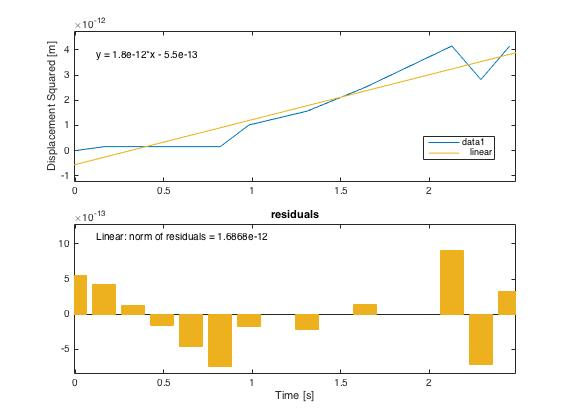
\includegraphics[width=0.50\textwidth]{plots/linear_fit.jpg}
\caption{The top panel shows a linear fit on the displacement data of a single particle undergoing Brownian diffusion. Shown in the bottom panels are the residuals from the linear fit. The residuals are relatively large due to noise in the data; however, since there is no systematic trend in the residual, a higher order fit is not necessary. The timeslice is cropped to a shorter region so that the linear trend could be more easily visualized.}
\label{linear_fit}
\end{figure}

\paragraph{Gaussian method} Since Brownian motion are governed by Markov processes and these processes are ``memory-less"  and random, we can fit the position function to a Gaussian. This offers us another way to compute the diffusion coefficient, as explained by \cite{grier}, by fitting a histogram of the particle displacement (Eq.\ref{displace}) to an expected Gaussian probability density function  (Eq. \ref{gaus})and then extracting the variance ($\sigma$) in the denominator to get the diffusion coefficient. 
\begin{equation}\label{displace}
x = | r(t+\tau)-r(t)|
\end{equation}
\begin{equation}
P(x|\tau) = \frac{1}{\sqrt{4\pi D \tau}} e^{-\frac{x^2}{4D\tau}}
\label{gaus}
\end{equation}
The diffusion coefficient from the Gaussian-fitting method is therefore equal to $\sigma/2\tau$. Since our $\tau$=0.1s, we ignore possible contributions from the long-time measurement contributions to the 2d$\sigma^2$ error term. Even though I thought that the Gaussian-fitting method would yield better result than the linear fit, due to a more complex functional form used to fit the probability density function, the Gaussian method actually doesn't perform as well as the linear fit.
\subsection{Molecular Motors}
\par Molecular motors such as Kinesin and Dynein are proteins that move by converting energy from ATP hydrolysis to mechanical motion. As shown in Fig. \ref{onion}, these molecular proteins typically``walk" along the microtubules within the cell. These molecular protein  uses energy from the hydrolysis of one ATP molecule to bind to the microtubles and uses this energy to make a ``step" by an iteration of bending itself and then relaxation of the microtubules that it is clinging on to progress forward. 
\begin{figure}[h]
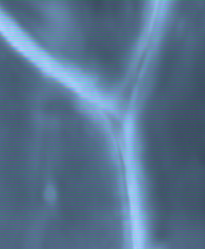
\includegraphics[width=0.20\textwidth]{plots/onion.png}
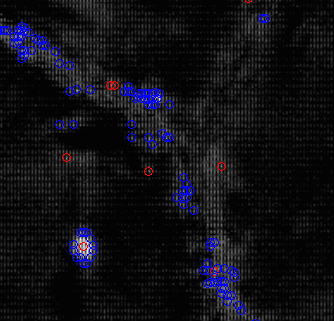
\includegraphics[width=0.25\textwidth]{plots/onion2.png}
\caption{(Left) Image of the onion cell under dark field illumination. (Right) We could see the an aggregate of detected particles flowing along the boundaries of the cell wall.}
\label{onion}
\end{figure}
\subsection{Intracellular transport}
\par I was unable to attain accurate measures for the bulk particle velocity of transport because the particle detected included those undergoing Brownian motion and those undergoing active transport. If we plot the histogram of velocities as shown in Fig. \ref{histo}, we attain a velocity measure of 2.569$\mu m$/s.
Using Stoke's law (Eq.\ref{stoke}), where $\nu$ is the viscosity of the cytosol, I determined that the frictional force for the transport of the particle is  $2.325\times 10^{-11}$ N. \cite{size} describes how different types of transport vesicles can range in size from 155nm to 560nm.  From the image, we counted that the cell spans approximately 1 to 2 pixels on our screen, which is is approximately 480nm and agrees with the aforementioned range of vesicle sizes. 
\begin{equation}
\label{stoke}
F_{fric} = 6\pi \nu r v
\end{equation}
\par Using W = F$\cdot$ d, where d is the distance of transport ($\approx$ size of the cell), we find that the work is 4.798$\times 10^{-16}$ J. The amount of energy that is released in the exothermic reaction where  ATP is hydrolyzed to ADP under normal conditions is around 83 zJ \citep{atp} and the motor efficiency is 60\%. The amount of work needed to transport a vesicle ($\approx 2.064\times10^{-5}m$) Due to the large uncertainty on the distance measures that we used, we got the non-sensical answer that the myosin motor can traverse the cell width in less than a step.
\par Another interesting observation is that the velocity is inadequately modelled by fitting a Gaussian. A Gaussian distribution is not a good fit because the goodness-of-fit chi squared is much larger than the chi squared of the Brownian example. This makes sense because the vesicle transport process is active rather than random, contrary to the case of Brownian motion in our microbead solutions. Since the vesicle is in a mesh or network, the motion is constrained along the tubules so that particle motion is not a random process. The velocity distribution of the onion cell sample is a mix of freely moving particle undergoing Brownian diffusion (in other parts of the cell) and constrained active transport, so we do not expect the onion cell transport velocities to be normally distributed. 
\begin{figure}[h]
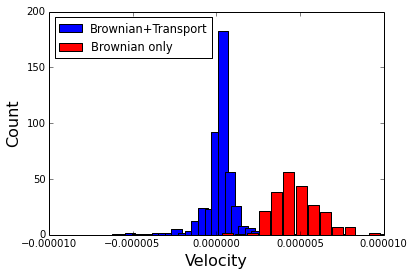
\includegraphics[width=0.50\textwidth]{plots/histo.png}
\caption{Velocity distributions of onion cell and microbead solution.}
\label{histo}
\end{figure} 
\par We assume that the error contributions from the measurement error for the pixel-to-meters conversion ratio ($\sigma_{pix}$) and the uncertainty on the velocity measurement  ($\sigma_{v}$) is independent, so we add the quadrature together ( $\sigma= \sqrt{\sigma_{pix}^2+\sigma_{v}^2}$) to get the uncertainty of the average velocity obtained. Therefore, the average velocity of a molecular protein in an onion cell is  v = 2.569$ \pm 1.011 \mu m/s$.
\section{Conclusion}\label{sec:conclusion}
%findings, future improvement? 
\par Jean Baptiste Perrin's experimental work on Brownian motion was of historical significance as it served as the one of the first experimental confirmation for the atomic nature of matter. In this lab, we replicated Perrin's experiment (with more advanced experimental technology) to investigate Brownian motion of  solutions of different microbead size and viscosity. We use the position, displacement and velocity information of particles undergoing Brownian diffusion to compute the diffusion coefficients of different solution. We employ three different analysis methods (Direct, Linear, and Gaussian) and found that the linear fit method agrees best with the theoretical estimates from our simulation. By looking at different solutions, we were able to confirm the relationship between the diffusion coefficient, particle size, and viscosity. We also analyzed the motion for a  molecular protein in a onion cell sample undergoing active intracellular transport, which had a non-Gaussian velocity distribution averaged around  at around v = 2.569$ \pm 1.011 \mu m/s$.

\acknowledgments
\section*{Acknowledgments}
I am sincerely thankful for support from Professor Harmut Haeffner, Kam-Biu Luk, Don Orlando, and my lab partner Xiyue Wang for contributing to successful completion of this lab.
\bibliography{bibdatabase}
%Raw Data: You must include the data that you took in lab in an appendix; the data should be clear enough so that someone could look at it and determine what you measured and how you measured it. You should be keeping a lab notebook, so simply photocopy all relevant pages. Your report should include all of the listed sections, along with the signed Pre-lab and Mid–Lab Discussion sheets.
\end{document}


